\documentclass[12pt,a4paper]{article}
\usepackage{amsmath, amssymb, geometry, booktabs, xcolor, hyperref,
            listings, pgfplots, tcolorbox, enumitem, fancyhdr, tikz, array}
\usepgfplotslibrary{fillbetween}
\geometry{margin=2.5cm}
\pgfplotsset{compat=1.18}
\tcbuselibrary{skins, breakable}

% Define custom environments
\newtcolorbox{curiositybox}[1]{colback=yellow!10, colframe=orange!80, title=#1, breakable}
\newtcolorbox{infobox}[1]{colback=blue!5, colframe=blue!60, title=#1, breakable}
\newtcolorbox{mistakebox}[1]{colback=red!5, colframe=red!60, title=#1, breakable}
\newtcolorbox{learnbox}[1]{colback=green!5, colframe=green!60, title=#1, breakable}

% Header and Footer
\pagestyle{fancy}
\fancyhf{}
\lhead{Optimization: Maxima, Minima, Lagrange Multipliers}
\rhead{Unit 4 -- LAC}
\cfoot{\thepage}

% Document Title Setup
\title{\textbf{Optimization: Maxima, Minima, and Lagrange Multipliers} \\ \large Unit 4 -- Multivariable Differentiation and Optimization}
\author{Department of Mathematics}
\date{\today}

\begin{document}
\maketitle
\tableofcontents
\newpage

%=============================================================
\section{Real-World Engineering Hook}
%=============================================================

\begin{curiositybox}{Why Should an Engineer Care?}
Imagine a structural engineer designing the cross-section of a steel beam for a bridge. The objective is to \emph{minimize the total material cost} (weight of steel) while the beam must still withstand a prescribed bending stress. If the engineer treats this as an unconstrained problem---ignoring the stress constraint---the optimiser returns a cross-section of zero area, which is mathematically optimal but physically catastrophic. The bridge collapses.

The same situation arises in rocket trajectory optimisation: NASA mission designers must maximise payload delivered to geostationary orbit subject to fuel-budget and re-entry-angle constraints. An unconstrained gradient search wanders off the feasible set and returns an answer that violates orbital mechanics. Similarly, antenna engineers shaping a parabolic reflector for a satellite dish minimise sidelobe radiation subject to a fixed aperture diameter constraint---miss the saddle point in the objective landscape and the dish radiates power in the wrong direction, losing the signal entirely.

\medskip
Three failure modes occur repeatedly in practice:
\begin{enumerate}
  \item Ignoring a \textbf{saddle point}: the algorithm declares ``minimum found'' at a point where the surface curves upward in one direction and downward in another---every nearby design direction seems safe until one load case exposes the flaw.
  \item Applying an \textbf{unconstrained} method to a \textbf{constrained} problem: the optimal unconstrained point lies outside the feasible region, so the returned design violates physical or regulatory limits.
  \item Misidentifying a \textbf{local minimum} as the \textbf{global minimum}: a lighter but weaker beam section satisfies local optimality conditions yet fails the overall safety factor requirement.
\end{enumerate}

The tools in this unit---critical-point analysis, the second-derivative (discriminant) test, and Lagrange multipliers---exist precisely to prevent these failures.
\end{curiositybox}

%=============================================================
\section{Why This Topic Exists}
%=============================================================

\begin{center}
\begin{tabular}{@{}lll@{}}
\toprule
\textbf{Sub-Topic} & \textbf{Core Mathematical Tool} & \textbf{Engineering Consequence} \\
\midrule
Critical Points & Set $\partial f/\partial x = 0$, $\partial f/\partial y = 0$ & Locate candidate optimal designs; miss them \\
 & simultaneously & and you never find the best beam or wing shape \\
\midrule
Discriminant Test & $D = f_{xx}f_{yy} - (f_{xy})^{2}$ & Distinguish load-bearing minimum from a \\
 & classification rules & dangerous saddle that will buckle under off-axis load \\
\midrule
Lagrange Multipliers & $\nabla f = \lambda \nabla g$, $g = 0$ & Optimise cost/weight/power under hard physical \\
 & (constrained system) & constraints such as fixed volume, stress limit, or budget \\
\bottomrule
\end{tabular}
\end{center}

\begin{learnbox}{Core Learning Objectives}
By the end of this unit you will be able to:
\begin{itemize}
  \item Find all critical points of a differentiable function $f(x,y)$ by solving the simultaneous equations $f_x = 0$ and $f_y = 0$.
  \item Apply the discriminant test to classify every critical point as a local maximum, local minimum, or saddle point.
  \item Handle the inconclusive case $D = 0$ using inspection or higher-order analysis.
  \item Set up and solve a Lagrange multiplier system for one equality constraint.
  \item Interpret the geometric meaning of Lagrange multipliers as level-curve tangency.
  \item Apply these methods to realistic engineering design and cost-minimisation problems.
\end{itemize}
\end{learnbox}

%=============================================================
\section{Intuition First \& Mathematical Definitions}
%=============================================================

\subsection{Maxima and Minima (Critical Points)}

Picture a hilly landscape. A local maximum is a hilltop---walk in any direction and you go downhill. A local minimum is a valley bottom---walk in any direction and you go uphill. At both points the ground is perfectly flat: the slope (gradient) is zero. For a surface $z = f(x,y)$, ``flat'' means both partial derivatives vanish simultaneously. These flat points are the candidates for optimal values, so we find them first before deciding what kind of extremum (if any) they represent.

\begin{infobox}{Critical Points of $f(x,y)$ --- Definitions and Conditions}
\textbf{Definition.} A point $(a,b)$ in the domain of $f(x,y)$ is called a \emph{critical point} (or stationary point) if
\[
  f_x(a,b) = \frac{\partial f}{\partial x}\bigg|_{(a,b)} = 0
  \quad \text{and} \quad
  f_y(a,b) = \frac{\partial f}{\partial y}\bigg|_{(a,b)} = 0.
\]

\textbf{Types of critical points (informal).}
\begin{itemize}
  \item \textbf{Local maximum}: $f(a,b) \geq f(x,y)$ for all $(x,y)$ near $(a,b)$.
  \item \textbf{Local minimum}: $f(a,b) \leq f(x,y)$ for all $(x,y)$ near $(a,b)$.
  \item \textbf{Saddle point}: neither a local max nor a local min; the surface curves upward in some directions and downward in others through $(a,b)$.
\end{itemize}

\textbf{Procedure to find critical points.}
\begin{enumerate}
  \item Compute $f_x = \partial f/\partial x$ and $f_y = \partial f/\partial y$.
  \item Set $f_x = 0$ and $f_y = 0$.
  \item Solve the resulting simultaneous system of equations for $(x,y)$.
  \item Each solution is a critical point candidate; classification follows in the next sub-topic.
\end{enumerate}

\textbf{Note.} Finding critical points only tells us \emph{where} to look. It does not yet tell us \emph{what kind} of extremum we have.
\end{infobox}

\textbf{Worked Example 1.1 --- Finding Critical Points of $f(x,y) = x^{2} + y^{2} - 4x - 6y + 20$.}

Step 1: Compute partial derivatives.
\[
  f_x = 2x - 4, \qquad f_y = 2y - 6.
\]

Step 2: Set both equal to zero.
\[
  2x - 4 = 0 \;\Rightarrow\; x = 2, \qquad 2y - 6 = 0 \;\Rightarrow\; y = 3.
\]

Step 3: The unique critical point is $(2, 3)$.

Step 4: Evaluate $f$ there: $f(2,3) = 4 + 9 - 8 - 18 + 20 = 7$.

So the function has a single critical point at $(2,3)$ with value $7$. Classification (minimum, maximum, or saddle) requires the discriminant test in the next subsection.

%-----------------------------------------------------------
\subsection{Second Derivative Test (Discriminant Method)}
%-----------------------------------------------------------

Once you have a critical point, you need to decide its nature. Think of the surface near the critical point as shaped like a bowl (minimum), an upside-down bowl (maximum), or a riding saddle (saddle point). The \emph{discriminant} $D$ captures this shape by comparing the curvatures in all directions simultaneously. It is the determinant of the Hessian matrix of second partial derivatives evaluated at the critical point.

\begin{infobox}{Discriminant (Second Derivative) Test --- Formula and Classification}
\textbf{Definition.} Given a function $f(x,y)$ with continuous second partial derivatives, define the \emph{discriminant} at a critical point $(a,b)$:
\[
  D(a,b) = f_{xx}(a,b)\,f_{yy}(a,b) - \bigl[f_{xy}(a,b)\bigr]^{2}.
\]

\textbf{Classification Table.}

\begin{center}
\begin{tabular}{@{}ccc@{}}
\toprule
\textbf{Condition} & \textbf{Extra condition} & \textbf{Classification} \\
\midrule
$D > 0$ & $f_{xx}(a,b) > 0$ & Local \textbf{minimum} \\
$D > 0$ & $f_{xx}(a,b) < 0$ & Local \textbf{maximum} \\
$D < 0$ & --- & \textbf{Saddle point} \\
$D = 0$ & --- & \textbf{Inconclusive}; higher-order analysis needed \\
\bottomrule
\end{tabular}
\end{center}

\textbf{Key formulas.}
\[
  f_{xx} = \frac{\partial^{2} f}{\partial x^{2}}, \quad
  f_{yy} = \frac{\partial^{2} f}{\partial y^{2}}, \quad
  f_{xy} = \frac{\partial^{2} f}{\partial x \partial y}.
\]

\textbf{Hessian matrix interpretation.}
\[
  H = \begin{pmatrix} f_{xx} & f_{xy} \\ f_{xy} & f_{yy} \end{pmatrix},
  \qquad D = \det(H).
\]
If $D > 0$, the Hessian is definite (both eigenvalues same sign); if $D < 0$, the Hessian is indefinite (eigenvalues of opposite sign, hence saddle).
\end{infobox}

\textbf{Worked Example 2.1 --- Classifying All Critical Points of $f(x,y) = x^{3} + y^{3} - 3x - 12y + 20$.}

Step 1: Partial derivatives.
\[
  f_x = 3x^{2} - 3, \qquad f_y = 3y^{2} - 12.
\]

Step 2: Set to zero.
\[
  3x^{2} - 3 = 0 \;\Rightarrow\; x^{2} = 1 \;\Rightarrow\; x = \pm 1.
\]
\[
  3y^{2} - 12 = 0 \;\Rightarrow\; y^{2} = 4 \;\Rightarrow\; y = \pm 2.
\]

Step 3: Four critical points: $(1,2)$, $(1,-2)$, $(-1,2)$, $(-1,-2)$.

Step 4: Second partial derivatives.
\[
  f_{xx} = 6x, \quad f_{yy} = 6y, \quad f_{xy} = 0.
\]

Step 5: Compute $D = f_{xx}f_{yy} - (f_{xy})^{2} = (6x)(6y) - 0 = 36xy$ at each point.

\begin{center}
\begin{tabular}{@{}cccccl@{}}
\toprule
Point & $f_{xx}$ & $f_{yy}$ & $f_{xy}$ & $D = 36xy$ & Classification \\
\midrule
$(1,2)$   & $6$  & $12$ & $0$ & $72 > 0$  & $f_{xx} = 6 > 0 \Rightarrow$ \textbf{Local minimum} \\
$(1,-2)$  & $6$  & $-12$& $0$ & $-72 < 0$ & \textbf{Saddle point} \\
$(-1,2)$  & $-6$ & $12$ & $0$ & $-72 < 0$ & \textbf{Saddle point} \\
$(-1,-2)$ & $-6$ & $-12$& $0$ & $72 > 0$  & $f_{xx} = -6 < 0 \Rightarrow$ \textbf{Local maximum} \\
\bottomrule
\end{tabular}
\end{center}

\medskip
\textbf{Worked Example 2.2 --- The Inconclusive Case $D = 0$ for $f(x,y) = x^{4} + y^{4} - 2x^{2}$.}

Step 1: Partial derivatives.
\[
  f_x = 4x^{3} - 4x = 4x(x^{2}-1), \qquad f_y = 4y^{3}.
\]

Step 2: Critical points.
\[
  4x(x^{2}-1) = 0 \;\Rightarrow\; x = 0, \pm 1; \qquad 4y^{3} = 0 \;\Rightarrow\; y = 0.
\]
Critical points: $(0,0)$, $(1,0)$, $(-1,0)$.

Step 3: Second derivatives.
\[
  f_{xx} = 12x^{2} - 4, \quad f_{yy} = 12y^{2}, \quad f_{xy} = 0.
\]

At $(0,0)$: $f_{xx} = -4$, $f_{yy} = 0$, $f_{xy} = 0$, so $D = (-4)(0) - 0 = 0$. \textbf{Inconclusive.}

Inspection: $f(x,0) = x^{4} - 2x^{2}$; near $x=0$, this equals $-2x^{2} < 0$ for small $x \neq 0$, while $f(0,0) = 0$. Also $f(0,y) = y^{4} \geq 0 = f(0,0)$. So the behaviour is not uniform in all directions. Checking along $x=0$: $f$ decreases; along $y=0$: $f$ has a local max at $x=0$. Thus $(0,0)$ is a \textbf{saddle point} (confirmed by inspection when $D=0$).

At $(1,0)$: $f_{xx} = 12-4 = 8$, $f_{yy} = 0$, $D = 0$. Inspect $f(1,y) = 1 + y^{4} - 2 = y^{4} - 1$, which has minimum at $y = 0$, i.e., $(1,0)$ is a local minimum in the $y$-direction. Check $f(x,0) = x^{4} - 2x^{2}$; local min at $x = 1$ since $\frac{d}{dx}(x^{4}-2x^{2}) = 4x^{3} - 4x = 0$ at $x=1$ and the second derivative $12x^{2}-4 = 8 > 0$. Hence $(1,0)$ is a \textbf{local minimum}. By symmetry, $(-1,0)$ is also a \textbf{local minimum}.

%-----------------------------------------------------------
\subsection{Lagrange Multipliers and Constrained Optimization}
%-----------------------------------------------------------

Imagine you are standing on a hilly surface and you are told you must stay on a fixed circular path drawn on the ground. You want to find the highest point on that path. You cannot simply take the unconstrained peak because it might lie off the path. The method of Lagrange multipliers says: at the constrained optimum, the hill's gradient (the direction of steepest ascent of $f$) must be exactly parallel to the constraint curve's gradient ($\nabla g$). If they were not parallel, you could slide along the constraint and go higher---contradicting optimality. This geometric tangency condition is precisely $\nabla f = \lambda \nabla g$.

\begin{infobox}{Method of Lagrange Multipliers --- One Constraint}
\textbf{Problem:} Maximise or minimise $f(x,y)$ subject to the constraint $g(x,y) = 0$.

\textbf{Lagrange Condition.} At an extremum $(a,b)$, there exists a scalar $\lambda$ (the \emph{Lagrange multiplier}) such that
\[
  \nabla f(a,b) = \lambda\, \nabla g(a,b),
\]
which expands to the system:
\[
  \frac{\partial f}{\partial x} = \lambda\,\frac{\partial g}{\partial x}, \qquad
  \frac{\partial f}{\partial y} = \lambda\,\frac{\partial g}{\partial y}, \qquad
  g(x,y) = 0.
\]
This gives \textbf{three equations} in three unknowns $(x, y, \lambda)$.

\textbf{Geometric interpretation.} The level curve $f(x,y) = c$ is tangent to the constraint curve $g(x,y) = 0$ at the optimal point. The two gradients are parallel (one is a scalar multiple of the other) because tangent lines of the two curves coincide.

\textbf{Extension to two constraints.} To optimise $f(x,y,z)$ subject to $g(x,y,z)=0$ and $h(x,y,z)=0$, solve:
\[
  \nabla f = \lambda\,\nabla g + \mu\,\nabla h, \quad g = 0, \quad h = 0.
\]
This gives \textbf{five equations} in five unknowns $(x,y,z,\lambda,\mu)$.

\textbf{Interpretation of $\lambda$.} The multiplier $\lambda$ measures the sensitivity of the optimal value $f^{*}$ to a relaxation of the constraint: $\lambda \approx \Delta f^{*} / \Delta c$ where $c$ is the right-hand side of the constraint $g = c$.

\textbf{Procedure (one constraint).}
\begin{enumerate}
  \item Write $L(x,y,\lambda) = f(x,y) - \lambda\,g(x,y)$ (the \emph{Lagrangian}).
  \item Set $\partial L/\partial x = 0$, $\partial L/\partial y = 0$, $\partial L/\partial \lambda = 0$.
  \item Solve the system for $(x, y, \lambda)$.
  \item Evaluate $f$ at each solution; compare to determine maximum/minimum.
\end{enumerate}
\end{infobox}

\textbf{Worked Example 3.1 --- Minimise $f(x,y) = x^{2} + y^{2}$ subject to $x + 2y = 5$.}

Step 1: Identify objective and constraint.
\[
  f(x,y) = x^{2} + y^{2}, \qquad g(x,y) = x + 2y - 5 = 0.
\]

Step 2: Compute gradients.
\[
  \nabla f = (2x,\, 2y), \qquad \nabla g = (1,\, 2).
\]

Step 3: Lagrange system $\nabla f = \lambda \nabla g$, $g = 0$:
\[
  2x = \lambda \cdot 1 \;\Rightarrow\; \lambda = 2x, \tag{i}
\]
\[
  2y = \lambda \cdot 2 \;\Rightarrow\; \lambda = y. \tag{ii}
\]
\[
  x + 2y = 5. \tag{iii}
\]

Step 4: From (i) and (ii): $2x = y$, so $y = 2x$.

Step 5: Substitute into (iii): $x + 2(2x) = 5 \Rightarrow 5x = 5 \Rightarrow x = 1$.

Step 6: $y = 2(1) = 2$, $\lambda = 2(1) = 2$.

Step 7: Optimal point is $(1,2)$.

Step 8: $f(1,2) = 1 + 4 = 5$.

\textbf{Interpretation.} The point $(1,2)$ is the point on the line $x + 2y = 5$ closest to the origin (since $x^{2}+y^{2}$ is the squared distance from the origin). The minimum distance is $\sqrt{5}$.

%=============================================================
\section{Visual Artifacts \& Geometric Interpretation}
%=============================================================

\subsection*{Figure 1: 3D Surface of $f(x,y) = x^{3} - 3x + y^{2}$ (Saddle and Local Minimum)}

\begin{center}
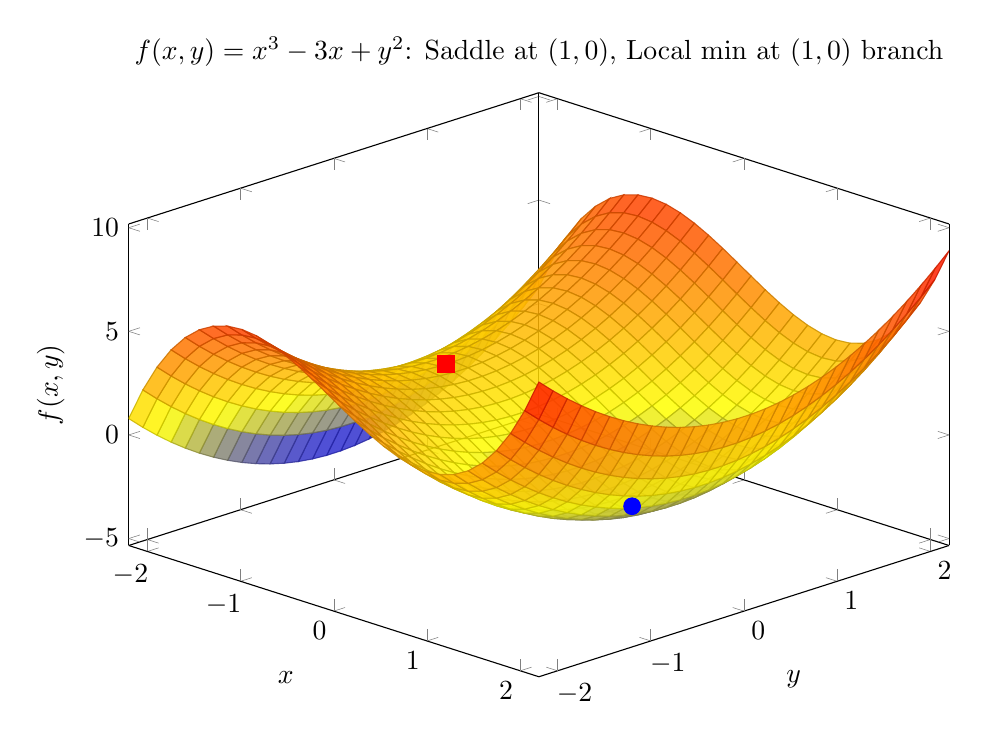
\begin{tikzpicture}
\begin{axis}[
  width=12cm, height=9cm,
  xlabel={$x$}, ylabel={$y$}, zlabel={$f(x,y)$},
  title={$f(x,y) = x^3 - 3x + y^2$: Saddle at $(1,0)$, Local min at $(1,0)$ branch},
  colormap/hot,
  view={45}{30},
  samples=30,
  domain=-2.2:2.2,
  y domain=-2.2:2.2,
]
\addplot3[surf, opacity=0.85] {x^3 - 3*x + y^2};
\addplot3[mark=*, mark size=3pt, color=blue] coordinates {(1,0,-2)};
\addplot3[mark=square*, mark size=3pt, color=red] coordinates {(-1,0,2)};
\end{axis}
\end{tikzpicture}
\end{center}

\noindent\textbf{Note.} The blue dot marks the local minimum at $(1,0)$ where $f = -2$; the red square marks the saddle point at $(-1,0)$ where $f = 2$.

\subsection*{Figure 2: Level Curves and Lagrange Multiplier Geometry}

\begin{center}
\begin{tikzpicture}
\begin{axis}[
  width=10cm, height=9cm,
  xlabel={$x$}, ylabel={$y$},
  title={Level Curves of $f(x,y)=x^2+y^2$ and Constraint $x+2y=5$},
  xmin=-1, xmax=5, ymin=-1, ymax=4,
  axis equal image,
  legend pos=north west,
]
% Level curves: circles x^2+y^2=c for c=5,10,15,20
\addplot[domain=0:360, samples=200, color=blue, thick]
  ({sqrt(5)*cos(x)}, {sqrt(5)*sin(x)});
\addplot[domain=0:360, samples=200, color=blue, dashed]
  ({sqrt(10)*cos(x)}, {sqrt(10)*sin(x)});
\addplot[domain=0:360, samples=200, color=blue, dotted]
  ({sqrt(15)*cos(x)}, {sqrt(15)*sin(x)});
% Constraint line x+2y=5
\addplot[domain=-1:5, color=red, thick] {(5-x)/2};
% Optimal point (1,2)
\addplot[mark=*, mark size=4pt, color=green!60!black] coordinates {(1,2)};
% Gradient arrows (schematic)
\draw[->, thick, orange] (axis cs:1,2) -- (axis cs:1.7,2.35) node[right]{\small $\nabla f$};
\draw[->, thick, purple] (axis cs:1,2) -- (axis cs:1.45,1.78) node[right]{\small $\nabla g$};
\legend{$f=5$ (optimal circle), $f=10$, $f=15$, Constraint $x+2y=5$, Optimal $(1,2)$}
\end{axis}
\end{tikzpicture}
\end{center}

\noindent\textbf{Geometric meaning.} At the constrained optimum $(1,2)$, the level curve $x^{2}+y^{2}=5$ is exactly tangent to the constraint line $x+2y=5$. The gradients $\nabla f$ and $\nabla g$ point in parallel directions, confirming $\nabla f = \lambda \nabla g$ with $\lambda = 2$.

\subsection*{Figure 3: Contour Plot of $f(x,y) = x^{3}+y^{3}-3x-12y+20$ with Critical Points}

\begin{center}
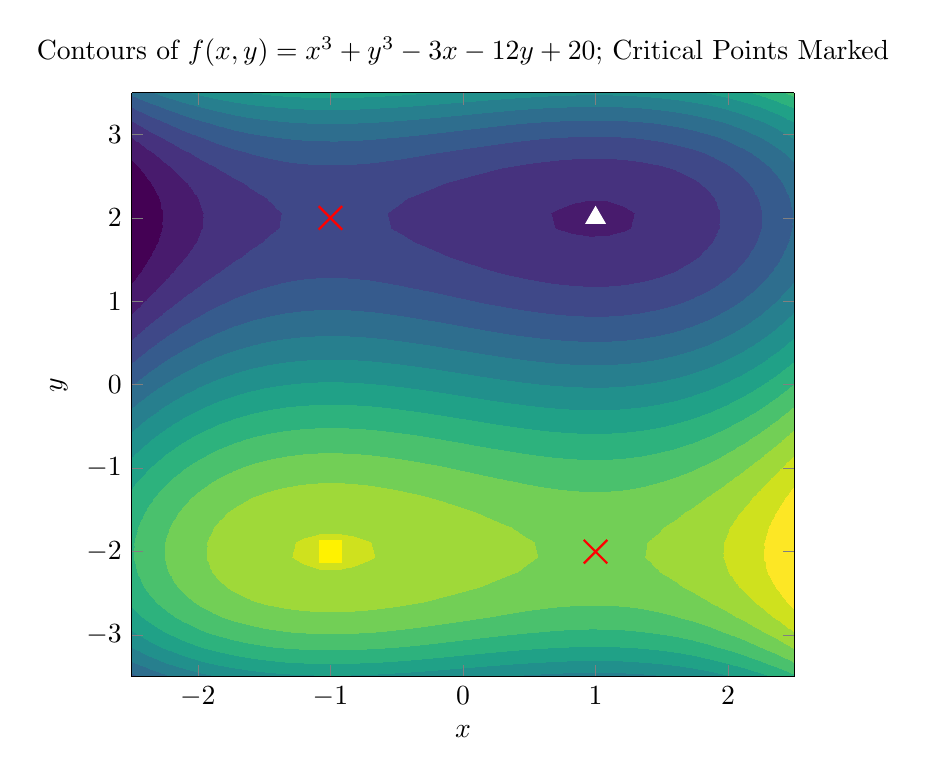
\begin{tikzpicture}
\begin{axis}[
  width=10cm, height=9cm,
  xlabel={$x$}, ylabel={$y$},
  title={Contours of $f(x,y)=x^3+y^3-3x-12y+20$; Critical Points Marked},
  view={0}{90},
  colormap/viridis,
  samples=40,
  domain=-2.5:2.5,
  y domain=-3.5:3.5,
]
\addplot3[contour filled={number=15}] {x^3+y^3-3*x-12*y+20};
\addplot[mark=triangle*, mark size=4pt, color=white] coordinates {(1,2)};
\addplot[mark=square*, mark size=4pt, color=yellow] coordinates {(-1,-2)};
\addplot[mark=x, mark size=6pt, color=red, thick] coordinates {(1,-2)};
\addplot[mark=x, mark size=6pt, color=red, thick] coordinates {(-1,2)};
\end{axis}
\end{tikzpicture}
\end{center}

\noindent White triangle: local minimum $(1,2)$. Yellow square: local maximum $(-1,-2)$. Red crosses: saddle points $(1,-2)$ and $(-1,2)$.

%=============================================================
\section{Step-by-Step Algorithmic Workflow}
%=============================================================

\subsection*{Workflow A: Unconstrained Optimisation}

\begin{infobox}{Algorithm --- Unconstrained Critical Point Analysis}
\begin{enumerate}
  \item \textbf{Compute} $f_x = \partial f/\partial x$ and $f_y = \partial f/\partial y$.
  \item \textbf{Solve} $f_x = 0$ and $f_y = 0$ simultaneously to find all critical points $(a_i, b_i)$.
  \item \textbf{Compute} second partial derivatives $f_{xx}$, $f_{yy}$, $f_{xy}$ at each critical point.
  \item \textbf{Evaluate discriminant} $D = f_{xx}f_{yy} - (f_{xy})^{2}$ at each critical point.
  \item \textbf{Classify} using the decision tree:
  \[
    D > 0 \;\Rightarrow\; \begin{cases} f_{xx} > 0: & \text{Local minimum} \\ f_{xx} < 0: & \text{Local maximum} \end{cases}; \quad D < 0 \Rightarrow \text{Saddle}; \quad D = 0 \Rightarrow \text{Inspect}.
  \]
  \item \textbf{Evaluate} $f(a_i, b_i)$ to find the optimal function value.
\end{enumerate}
\end{infobox}

\subsection*{Workflow B: Constrained Optimisation via Lagrange Multipliers}

\begin{infobox}{Algorithm --- Lagrange Multiplier Method (One Constraint)}
\begin{enumerate}
  \item \textbf{Identify} objective $f(x,y)$ and constraint $g(x,y) = 0$.
  \item \textbf{Compute} $\nabla f = (f_x, f_y)$ and $\nabla g = (g_x, g_y)$.
  \item \textbf{Write} the Lagrange system:
    \[
      f_x = \lambda g_x, \quad f_y = \lambda g_y, \quad g(x,y) = 0.
    \]
  \item \textbf{Solve} for $(x, y, \lambda)$. (Typically: eliminate $\lambda$ from the first two equations, substitute into the third.)
  \item \textbf{Evaluate} $f$ at each solution point.
  \item \textbf{Compare} values: the largest is the constrained maximum; smallest is the constrained minimum.
  \item \textbf{Interpret} $\lambda$: it equals $df^{*}/dc$ where $c$ is the constraint right-hand side. A large $|\lambda|$ means the optimal value is very sensitive to the constraint.
\end{enumerate}
\end{infobox}

\subsection*{Decision Tree for Discriminant}

\begin{center}
\begin{tikzpicture}[
  node distance=1.6cm,
  every node/.style={draw, rounded corners, align=center, font=\small},
  decision/.style={diamond, aspect=2, draw, align=center},
  result/.style={rectangle, draw, fill=green!20}
]
\node (start) {Critical point $(a,b)$ found};
\node [decision, below=of start] (D) {Compute $D$};
\node [result, below left=1.4cm and 2.5cm of D] (saddle) {$D < 0$\\Saddle point};
\node [decision, below=1.8cm of D] (Dg0) {$D > 0$?};
\node [result, below left=1.4cm and 2cm of Dg0] (min) {$f_{xx} > 0$\\Local minimum};
\node [result, below right=1.4cm and 2cm of Dg0] (max) {$f_{xx} < 0$\\Local maximum};
\node [result, below right=1.4cm and 2.5cm of D] (inc) {$D = 0$\\Inconclusive:\\inspect or\\higher-order test};
\draw[->] (start) -- (D);
\draw[->] (D) -- node[left,draw=none]{$D < 0$} (saddle);
\draw[->] (D) -- node[right,draw=none]{$D > 0$} (Dg0);
\draw[->] (D) -- node[right,draw=none]{$D = 0$} (inc);
\draw[->] (Dg0) -- node[left,draw=none]{$f_{xx}>0$} (min);
\draw[->] (Dg0) -- node[right,draw=none]{$f_{xx}<0$} (max);
\end{tikzpicture}
\end{center}

%=============================================================
\section{Fully Worked Step-by-Step Numerical Examples}
%=============================================================

\subsection*{Example 1: Find and Classify All Critical Points of $f(x,y) = x^{3} + y^{3} - 3x - 12y + 20$}

\textbf{Step 1.} Compute first partial derivatives.
\[
  f_x = 3x^{2} - 3, \qquad f_y = 3y^{2} - 12.
\]

\textbf{Step 2.} Set each equal to zero.
\[
  3x^{2} - 3 = 0 \;\Rightarrow\; x^{2} = 1 \;\Rightarrow\; x = 1 \text{ or } x = -1.
\]
\[
  3y^{2} - 12 = 0 \;\Rightarrow\; y^{2} = 4 \;\Rightarrow\; y = 2 \text{ or } y = -2.
\]

\textbf{Step 3.} Critical points: $(1,2)$, $(1,-2)$, $(-1,2)$, $(-1,-2)$.

\textbf{Step 4.} Second partial derivatives.
\[
  f_{xx} = 6x, \quad f_{yy} = 6y, \quad f_{xy} = 0.
\]

\textbf{Step 5.} Discriminant $D = f_{xx}f_{yy} - (f_{xy})^{2} = 36xy$.

\textbf{Step 6.} Classification table.

\begin{center}
\begin{tabular}{@{}cccccl@{}}
\toprule
Point & $f_{xx}$ & $f_{yy}$ & $D$ & $f$ value & Classification \\
\midrule
$(1,2)$   & $6$  & $12$  & $72 > 0$  & $1+8-3-24+20 = 2$  & Local \textbf{minimum} ($f_{xx}>0$) \\
$(1,-2)$  & $6$  & $-12$ & $-72 < 0$ & $1-8-3+24+20 = 34$ & \textbf{Saddle point} \\
$(-1,2)$  & $-6$ & $12$  & $-72 < 0$ & $-1+8+3-24+20 = 6$ & \textbf{Saddle point} \\
$(-1,-2)$ & $-6$ & $-12$ & $72 > 0$  & $-1-8+3+24+20 = 38$& Local \textbf{maximum} ($f_{xx}<0$) \\
\bottomrule
\end{tabular}
\end{center}

\textbf{Conclusion.} Local minimum at $(1,2)$ with $f = 2$; local maximum at $(-1,-2)$ with $f = 38$; saddle points at $(1,-2)$ and $(-1,2)$.

\subsection*{Example 2: Inconclusive Case --- $f(x,y) = x^{4} + y^{4} - 2x^{2}$}

\textbf{Step 1.}
\[
  f_x = 4x^{3} - 4x = 4x(x-1)(x+1), \qquad f_y = 4y^{3}.
\]

\textbf{Step 2.} $f_x = 0 \Rightarrow x = 0, 1, -1$. \quad $f_y = 0 \Rightarrow y = 0$.

\textbf{Step 3.} Critical points: $(0,0)$, $(1,0)$, $(-1,0)$.

\textbf{Step 4.}
\[
  f_{xx} = 12x^{2} - 4, \quad f_{yy} = 12y^{2}, \quad f_{xy} = 0.
\]

At $(0,0)$: $f_{xx} = -4$, $f_{yy} = 0$, $D = (-4)(0) - 0 = 0$. \textbf{Inconclusive.}

At $(1,0)$: $f_{xx} = 8$, $f_{yy} = 0$, $D = 0$. \textbf{Inconclusive.}

At $(-1,0)$: $f_{xx} = 8$, $f_{yy} = 0$, $D = 0$. \textbf{Inconclusive.}

\textbf{Step 5: Inspection for $(0,0)$.}

Along $y = 0$: $f(x,0) = x^{4} - 2x^{2}$. Near $x = 0$: $f \approx -2x^{2} < 0 = f(0,0)$ for $x \neq 0$ small.

Along $x = 0$: $f(0,y) = y^{4} \geq 0 = f(0,0)$ for all $y$.

Since $f$ decreases in the $x$-direction and increases in the $y$-direction from $(0,0)$, the point $(0,0)$ is a \textbf{saddle point}.

\textbf{Step 6: Inspection for $(1,0)$.}

$f(1,0) = 1 + 0 - 2 = -1$.

Along $y = 0$: $\frac{d}{dx}(x^{4}-2x^{2})\big|_{x=1} = 4-4 = 0$; $\frac{d^{2}}{dx^{2}}(x^{4}-2x^{2})\big|_{x=1} = 12-4 = 8 > 0$. So $(1,0)$ is a local minimum along $x$-axis.

Along $x = 1$: $f(1,y) = 1 + y^{4} - 2 = y^{4} - 1$, minimum at $y=0$. So $(1,0)$ is a local minimum along $y$-axis.

Since $f(x,y) \geq f(1,0)$ in all directions around $(1,0)$, it is a \textbf{local minimum with $f = -1$}. By symmetry, $(-1,0)$ is also a \textbf{local minimum with $f = -1$}.

\subsection*{Example 3 (Engineering): Minimise Surface Area of an Open Rectangular Box with Volume $8\ \mathrm{m}^{3}$}

\textbf{Problem setup.} A rectangular box (no lid) has dimensions $x$ (length), $y$ (width), $z$ (height). Minimise the surface area $S = xy + 2xz + 2yz$ subject to the volume constraint $V = xyz = 8$.

\textbf{Step 1.} Express $z$ from the constraint.
\[
  xyz = 8 \;\Rightarrow\; z = \frac{8}{xy}.
\]

\textbf{Step 2.} Substitute into $S$.
\[
  S(x,y) = xy + 2x\cdot\frac{8}{xy} + 2y\cdot\frac{8}{xy}
          = xy + \frac{16}{y} + \frac{16}{x}.
\]

\textbf{Step 3.} Set partial derivatives to zero.
\[
  S_x = y - \frac{16}{x^{2}} = 0 \;\Rightarrow\; y = \frac{16}{x^{2}}. \tag{A}
\]
\[
  S_y = x - \frac{16}{y^{2}} = 0 \;\Rightarrow\; x = \frac{16}{y^{2}}. \tag{B}
\]

\textbf{Step 4.} From (A): $y = 16/x^{2}$. Substitute into (B):
\[
  x = \frac{16}{(16/x^{2})^{2}} = \frac{16 x^{4}}{256} = \frac{x^{4}}{16}.
\]
\[
  16x = x^{4} \;\Rightarrow\; x^{3} = 16 \;\Rightarrow\; x = 16^{1/3} = 2^{4/3}\ \mathrm{m}.
\]

\textbf{Step 5.} $y = 16/(2^{4/3})^{2} = 16/2^{8/3} = 2^{4}/2^{8/3} = 2^{4-8/3} = 2^{4/3}\ \mathrm{m}$.

\textbf{Step 6.} $z = 8/(x\cdot y) = 8/(2^{4/3}\cdot 2^{4/3}) = 8/2^{8/3} = 2^{3}/2^{8/3} = 2^{1/3}\ \mathrm{m}$.

Numerically: $2^{4/3} \approx 2.520\ \mathrm{m}$, $z = 2^{1/3} \approx 1.260\ \mathrm{m}$.

\textbf{Step 7.} Minimum surface area:
\[
  S = xy + \frac{16}{y} + \frac{16}{x}
  = (2^{4/3})^{2} + \frac{16}{2^{4/3}} + \frac{16}{2^{4/3}}
  = 2^{8/3} + 2 \cdot 2^{4} \cdot 2^{-4/3}
  = 2^{8/3} + 2^{5} \cdot 2^{-4/3}
  = 2^{8/3} + 2^{5-4/3}.
\]
\[
  = 2^{8/3} + 2^{11/3}
  = 2^{8/3}(1 + 2)
  = 3 \cdot 2^{8/3} \approx 3 \times 6.35 \approx 19.05\ \mathrm{m}^{2}.
\]

\textbf{Engineering Interpretation.} The optimal open box has a square base ($x = y \approx 2.52\ \mathrm{m}$) and a height that is exactly half the base length ($z \approx 1.26\ \mathrm{m} = x/2$). This square-base, half-height ratio is the cost-minimising shape for any open rectangular container of fixed volume---a result used directly in sheet-metal fabrication and packaging design.

%=============================================================
\section{Tabular Comparison / Workflow Reference}
%=============================================================

\begin{center}
\begin{tabular}{@{}p{3cm}p{5cm}p{5cm}@{}}
\toprule
\textbf{Feature} & \textbf{Unconstrained (Critical Point + Discriminant)} & \textbf{Constrained (Lagrange Multipliers)} \\
\midrule
\textbf{When to use} & No restrictions on $(x,y)$; objective has interior optimum & Equality constraint $g(x,y)=0$ must hold \\
\midrule
\textbf{Equation setup} & $f_x = 0$, $f_y = 0$ & $f_x = \lambda g_x$, $f_y = \lambda g_y$, $g = 0$ \\
\midrule
\textbf{No. of equations} & 2 equations, 2 unknowns & 3 equations, 3 unknowns $(x,y,\lambda)$ \\
\midrule
\textbf{Classification tool} & Discriminant $D = f_{xx}f_{yy}-(f_{xy})^2$ & Compare $f$ values at all solution points \\
\midrule
\textbf{Saddle interpretation} & $D < 0$ at critical point & No standard ``saddle'' test; must compare $f$ values \\
\midrule
\textbf{Multiplier meaning} & No multiplier & $\lambda = df^*/dc$; sensitivity to constraint \\
\midrule
\textbf{Inconclusive case} & $D = 0$; inspect or use higher-order test & Degenerate if $\nabla g = 0$ at solution \\
\midrule
\textbf{Engineering example} & Optimal antenna cross-section, free shape & Minimal-material beam under stress limit; box with fixed volume \\
\bottomrule
\end{tabular}
\end{center}

%=============================================================
\section{Common Student Mistakes \& Pitfalls}
%=============================================================

\begin{mistakebox}{Common Mistakes in Optimisation}
\begin{tabular}{@{}p{4.5cm}p{4.5cm}p{4.5cm}@{}}
\toprule
\textbf{Mistake} & \textbf{What goes wrong} & \textbf{Correct approach} \\
\midrule
\textbf{[Sub-topic 1]} Setting only $f_x = 0$, ignoring $f_y = 0$ & You find a curve of points, not individual critical points; classification is impossible & Always solve $f_x = 0$ and $f_y = 0$ \emph{simultaneously} as a system \\
\midrule
\textbf{[Sub-topic 1]} Forgetting to check all solutions when equations factor & E.g., $x(x-1)=0$ gives $x=0$ AND $x=1$; missing one gives an incomplete set of critical points & Fully factor or use the quadratic formula; list \emph{every} root \\
\midrule
\textbf{[Sub-topic 2]} Writing $D = f_{xx}f_{yy} + (f_{xy})^2$ (wrong sign) & Sign error flips the classification; saddles become minima and vice versa & Memorise $D = f_{xx}f_{yy} - (f_{xy})^2$ as a determinant; the minus sign is essential \\
\midrule
\textbf{[Sub-topic 2]} Concluding ``local minimum'' when $D = 0$ & $D = 0$ is the inconclusive case; the point might be a saddle or an inflection & Inspect $f$ along coordinate directions or use higher-order Taylor terms \\
\midrule
\textbf{[Sub-topic 2]} Checking only one direction when $D = 0$ & Along one axis the point looks like a min; along another it might decrease & Check behaviour in at least two independent directions (e.g., $y=0$ and $x=0$) \\
\midrule
\textbf{[Sub-topic 3]} Forgetting the constraint equation $g = 0$ in the Lagrange system & Without $g=0$ the system has infinitely many solutions; $\lambda$ is undetermined & The Lagrange system is always 3 equations: $f_x=\lambda g_x$, $f_y=\lambda g_y$, \emph{and} $g=0$ \\
\midrule
\textbf{[Sub-topic 3]} Discarding $\lambda$ after solving and not using it for checking & Losing $\lambda$ means no sensitivity analysis and no check on correctness & Keep $\lambda$; verify the solution satisfies all three equations \\
\midrule
\textbf{[Sub-topic 3]} Treating a constrained minimum as a global minimum & The Lagrange method finds a local constrained extremum; there may be other local optima or boundary effects & Evaluate $f$ at \emph{all} Lagrange solutions and compare; examine boundary or unboundedness if relevant \\
\bottomrule
\end{tabular}
\end{mistakebox}

%=============================================================
\section{Comprehensive Assessment Suite}
%=============================================================

\subsection*{Viva-Voce Questions}

\begin{enumerate}

  \item \textbf{[Sub-topic 1]} What is a critical point of a function $f(x,y)$? Write the two conditions that must hold simultaneously.

  \item \textbf{[Sub-topic 1]} Can a function have infinitely many critical points? Give an example of a function of two variables where every point on a line is a critical point.

  \item \textbf{[Sub-topic 2]} State the discriminant test for classifying a critical point $(a,b)$ of $f(x,y)$. What does each case ($D>0$, $D<0$, $D=0$) imply?

  \item \textbf{[Sub-topic 2]} Give a geometric interpretation of a saddle point. In what physical situation would an engineer encounter a saddle point in an objective function?

  \item \textbf{[Sub-topic 2]} Why is the case $D = 0$ called inconclusive? Describe one method to handle it.

  \item \textbf{[Sub-topic 3]} State the method of Lagrange multipliers for optimising $f(x,y)$ subject to $g(x,y) = 0$. How many equations does the system involve, and what are the unknowns?

  \item \textbf{[Sub-topic 3]} What does the Lagrange multiplier $\lambda$ represent physically? If you are minimising cost subject to a production constraint, what does a large $|\lambda|$ indicate?

  \item \textbf{[Sub-topic 3]} Explain geometrically why $\nabla f = \lambda \nabla g$ at a constrained optimum.

\end{enumerate}

\subsection*{Descriptive Exam Questions}

\begin{enumerate}

  \item Find and classify all critical points of $f(x,y) = 2x^{3} + 3y^{2} - 12x - 18y + 5$ using the discriminant test. Show all computations in full.

  \item Find the critical points of $f(x,y) = x^{2}y + xy^{2} - 4xy$. For each critical point, compute $D$ and classify as local maximum, local minimum, or saddle point. \textit{Hint: the critical points include $(0,0)$, $(2,0)$, $(0,2)$, and $(4/3, 4/3)$.}

  \item Using the method of Lagrange multipliers, find the maximum and minimum values of $f(x,y) = 3x + 4y$ on the circle $x^{2} + y^{2} = 25$. Verify by comparing all solution values.

  \item A manufacturer wants to build a closed rectangular box of volume $V = 64\ \mathrm{m}^{3}$ using the minimum possible surface area. Using Lagrange multipliers, find the optimal dimensions. State the minimum surface area and interpret the shape.

  \item Show that the function $f(x,y) = x^{2} - xy + y^{2} - 2x + y$ has exactly one critical point. Determine its nature using the discriminant test, find the minimum value, and describe what happens geometrically.

\end{enumerate}

\subsection*{Multiple Choice Questions}

\begin{enumerate}

  \item \textbf{[Sub-topic 1]} The critical points of $f(x,y) = x^{2} + 2y^{2} - 4x + 8y + 1$ are:
  \begin{enumerate}[label=(\Alph*)]
    \item $(1, 4)$
    \item \textbf{$(2, -2)$}
    \item $(4, -8)$
    \item $(0, 0)$
  \end{enumerate}
  \textit{Explanation:} $f_x = 2x-4 = 0 \Rightarrow x=2$; $f_y = 4y+8 = 0 \Rightarrow y=-2$. So $(2,-2)$ is the unique critical point.

  \item \textbf{[Sub-topic 2]} At a critical point $(a,b)$, if $D = f_{xx}f_{yy}-(f_{xy})^{2} = 25$ and $f_{xx}(a,b) = -5$, the point is a:
  \begin{enumerate}[label=(\Alph*)]
    \item Local minimum
    \item Saddle point
    \item \textbf{Local maximum}
    \item Inconclusive
  \end{enumerate}
  \textit{Explanation:} $D > 0$ and $f_{xx} < 0$ implies local maximum by the second derivative test.

  \item \textbf{[Sub-topic 2]} If $D = 0$ at a critical point, which of the following is correct?
  \begin{enumerate}[label=(\Alph*)]
    \item The point is always a saddle point
    \item The point is always a local minimum
    \item \textbf{The test is inconclusive; further analysis is needed}
    \item The point is not a critical point
  \end{enumerate}
  \textit{Explanation:} $D=0$ is the inconclusive case; inspection or higher-order methods must be used.

  \item \textbf{[Sub-topic 3]} The method of Lagrange multipliers converts the problem ``maximise $f(x,y)$ subject to $g(x,y)=0$'' into:
  \begin{enumerate}[label=(\Alph*)]
    \item A two-equation unconstrained system
    \item \textbf{A three-equation system in $(x,y,\lambda)$}
    \item A system of differential equations
    \item A two-variable unconstrained optimisation of the Lagrangian
  \end{enumerate}
  \textit{Explanation:} The system $f_x = \lambda g_x$, $f_y = \lambda g_y$, $g(x,y) = 0$ has three equations and three unknowns.

  \item \textbf{[Sub-topic 3]} When optimising $f(x,y) = x^{2}+y^{2}$ subject to $x+y = 4$ using Lagrange multipliers, the optimal point is:
  \begin{enumerate}[label=(\Alph*)]
    \item $(4, 0)$
    \item $(0, 4)$
    \item \textbf{$(2, 2)$}
    \item $(1, 3)$
  \end{enumerate}
  \textit{Explanation:} $\nabla f = \lambda \nabla g$: $2x = \lambda$, $2y = \lambda$, so $x=y$. Substituting into $x+y=4$: $2x=4 \Rightarrow x=y=2$.

  \item \textbf{[Sub-topic 1 \& 2]} For $f(x,y) = 4xy - x^{4} - y^{4}$, the discriminant $D$ at the critical point $(1,1)$ equals:
  \begin{enumerate}[label=(\Alph*)]
    \item $-12$
    \item $0$
    \item $16$
    \item \textbf{$128$}
  \end{enumerate}
  \textit{Explanation:} $f_{xx}=-12x^{2}$, $f_{yy}=-12y^{2}$, $f_{xy}=4$. At $(1,1)$: $D=(-12)(-12)-16=144-16=128>0$, $f_{xx}<0$: local maximum.

\end{enumerate}

%=============================================================
\section{Quick Recap \& Formula Sheet}
%=============================================================

\begin{learnbox}{Unit 4 Optimisation --- Formula Sheet and Key Takeaways}
\begin{itemize}
  \item \textbf{Critical point conditions:} $(a,b)$ is a critical point if $f_x(a,b)=0$ and $f_y(a,b)=0$ simultaneously; these are necessary but not sufficient for a local extremum.
  \item \textbf{Discriminant formula:} $D(a,b) = f_{xx}(a,b)\,f_{yy}(a,b) - [f_{xy}(a,b)]^{2} = \det(H)$ where $H$ is the Hessian matrix of $f$.
  \item \textbf{Classification rule:} $D > 0, f_{xx} > 0 \Rightarrow$ local min; $D > 0, f_{xx} < 0 \Rightarrow$ local max; $D < 0 \Rightarrow$ saddle; $D = 0 \Rightarrow$ inconclusive (inspect or use higher-order test).
  \item \textbf{Lagrange multiplier system (one constraint):} $f_x = \lambda g_x$, $f_y = \lambda g_y$, $g(x,y) = 0$ --- always three equations, three unknowns; eliminate $\lambda$ from the first two, then use the constraint.
  \item \textbf{Geometric meaning of Lagrange:} At the constrained optimum the level curve of $f$ is tangent to the constraint curve; equivalently, $\nabla f \parallel \nabla g$ (one is a scalar multiple of the other).
  \item \textbf{Multiplier interpretation:} $\lambda = df^*/dc$ measures sensitivity of the optimal value to relaxation of the constraint $g = c$; large $|\lambda|$ means the constraint is binding and costly.
  \item \textbf{When to use each method:} Unconstrained (discriminant) when the domain is open and free; Lagrange multipliers when there is a hard equality constraint that the optimal point must lie on.
  \item \textbf{Engineering takeaway:} Optimal open box with volume $V$ has a square base with $x = y = (2V)^{1/3}$ and height $z = x/2$; the square-base, half-height ratio minimises surface area for any volume.
\end{itemize}
\end{learnbox}

\end{document}
